% =====================================================================
%  Laborbericht 1 -- Biosignalverarbeitung
%  Aufbau der Hardware & Datenakquise
%
%  Aufgebaut nach Vorlagen/laborbericht.tex (MCI-LaTeX-Vorlage V3.0):
%  gleiche Dokumentklasse, % =====================================================================
%  definitions.tex -- angepasste Kopie von Vorlagen/definitions.tex
%  (MCI-Vorlage V3.0, Drauschke/Teschl/Mehrle)
%
%  Layout, Farben, Überschriften, Abstände und Verzeichnisnamen sind
%  unverändert übernommen. Geändert wurde nur, was mit pdflatex /
%  aktuellem TeX Live nicht mehr kompiliert:
%    - "german"           -> babel/ngerman + UTF-8 (Umlaute direkt tippen)
%    - graphicx[dvips]    -> graphicx (pdflatex kann PNG/PDF einbinden)
%    - pst-all, wallpaper, pgfplots, units, subfigure entfernt
%      (Konflikte \unit/\ang, nur für latex+dvips gedacht, nicht benötigt)
%    - PSTricks-Makros (Netzwerk-/Blocksymbole) entfernt
%  Ergänzt: booktabs, listings, \todo für offene Stellen.
% =====================================================================

\ifthenelse{\boolean{english}}
  {\usepackage[english]{babel}}
  {\usepackage[ngerman]{babel}}
\usepackage[utf8]{inputenc}
\usepackage[T1]{fontenc}
\usepackage{lmodern}
\usepackage{graphicx}
\usepackage[tmargin=1in,bmargin=1in,lmargin=1.25in,rmargin=1.25in]{geometry}
\usepackage{titlesec}
\usepackage{xcolor}
\usepackage[overload]{textcase}
\definecolor{MSBlue}{rgb}{.204,.353,.541}
\definecolor{MSLightBlue}{rgb}{.31,.506,.741}
% Set formats for each heading level (Abschnitte klein geschrieben wie in der Vorlage)
\titleformat{\section}[hang]{\rmfamily\bfseries\huge\color{MSBlue}}{\thesection}{1em}{\MakeLowercase}[]
\titleformat{\subsection}{\large\bfseries\sffamily\uppercase}{\thesubsection}{1em}{}
\titleformat{\subsubsection}{\sffamily\bfseries}{\thesubsubsection}{1em}{}
% babel überschreibt die Namen bei \begin{document}, daher erst dort setzen
% (\ifthenelse außerhalb, weil \MakeLowercase es in der Überschrift nicht verträgt)
\ifthenelse{\boolean{english}}
  {\AtBeginDocument{%
    \renewcommand\contentsname{table of contents.}%
    \renewcommand\listfigurename{list of figures.}%
    \renewcommand\listtablename{list of tables.}%
    \renewcommand\refname{\litname.}}}
  {\AtBeginDocument{%
    \renewcommand\contentsname{inhaltsverzeichnis.}%
    \renewcommand\listfigurename{abbildungsverzeichnis.}%
    \renewcommand\listtablename{tabellenverzeichnis.}%
    \renewcommand\refname{\litname.}}}
\usepackage{exscale,relsize}
\usepackage{fancyhdr}
\usepackage[small]{caption}
\usepackage{float}
\usepackage{amsmath}
\usepackage{amssymb}
\usepackage{rotating}
\usepackage{mathrsfs}
\usepackage{booktabs}
\usepackage{listings}
\setlength{\emergencystretch}{2em}

\newcommand{\babel}[2]{\ifthenelse{\boolean{english}}{#1}{#2}}

% auxillary symbols
\newcommand{\define}{\stackrel{!}{=}}
\renewcommand{\equiv}{\,\widehat{=}\,}
\newcommand{\subsubsubsection}{\textbf}
\newcommand{\mif}{\quad\mathrm{\babel{if}{falls}}\quad}
\newcommand{\with}{\quad\mathrm{\babel{with}{mit}}\quad}
\newcommand{\for}{\quad\mathrm{\babel{for}{für}}\quad}
\newcommand{\matlab}{MATLAB}

% format specifications
\renewcommand{\emph}{\textbf}
\newcommand{\file}{\textit}
\newcommand{\cmd}{\texttt}
\newcommand{\ten}{\boldsymbol}
\newcommand{\lemma}{\textit}

% Pfade zu Grafiken
\graphicspath{{abbildungen/}{../Abgabe_Lab1/figures/}}

% mathematical operators
\newcommand{\grad}{\,\mathrm{grad}\,}
\renewcommand{\div}{\,\mathrm{div}\,}
\newcommand{\rot}{\,\mathrm{rot}\,}
\newcommand{\lap}{\Delta}
\newcommand{\laplace}[1]{\mathscr{L}\left\{#1\right\}}
\newcommand{\trans}{^T}

\setlength{\parindent}{0em}
\setlength{\parskip}{1.5ex plus0.5ex minus0.5ex}
\setlength{\captionmargin}{3em}

% Quellcode (für Ausschnitte und Anhang)
\lstset{basicstyle=\ttfamily\footnotesize,frame=single,columns=fullflexible,
        keywordstyle=\bfseries,language=C++,breaklines=true}

% Offene Stellen rot markieren -- vor der Abgabe müssen alle weg sein
\newcommand{\todo}[1]{\textcolor{red}{\textbf{[TODO:} #1\textbf{]}}}
 und % Deckblatt:
\thispagestyle{empty}
\sffamily
%\put(-30,-685){\includegraphics[width=1.15\linewidth]{BG}}

{\bfseries


\vspace*{1cm}

\def\thesis{\ifthenelse{\boolean{english}}{laboratory report}{laborbericht}}
\textcolor{MSBlue}{\rmfamily\bfseries\huge\thesis.}%

\vspace*{0.5cm}

\textbf{\labtitle{ }(\labcode)}

\labname

\ifthenelse{\boolean{english}}{Lab}{Labor} \labnum

\vspace*{10cm}

\textcolor{gray}{\study}

\def\termname{\ifthenelse{\boolean{english}}{semester}{Semester}}
\textcolor{gray}{\term{ }\termname}

\def\lecturername{\ifthenelse{\boolean{english}}{Responsible lecturer}{Lehrveranstaltungsleiter}}
\textcolor{gray}{\lecturername: \lecturer}

\def\groupname{\ifthenelse{\boolean{english}}{Group}{Jahrgang}}
\textcolor{gray}{\groupname: \group}

\def\authorname{\ifthenelse{\boolean{english}}{Author}{Verfasser}}
\textcolor{gray}{\authorname: \student}

\textcolor{gray}{\today}

\newpage}
,
%  Gliederung der Vorlage, Literatur per BibTeX (IEEEtran + Literatur.bib).
%
%  Kompilieren:  latexmk -pdf laborbericht.tex
%  Max. 10 Seiten (inkl. Deckblatt).
% =====================================================================

\documentclass[a4paper,oneside,10pt]{article}

\usepackage{ifthen}
\newboolean{english}
%\setboolean{english}{true}		% auskommentieren fuer deutsche Version

% =====================================================================
%  definitions.tex -- angepasste Kopie von Vorlagen/definitions.tex
%  (MCI-Vorlage V3.0, Drauschke/Teschl/Mehrle)
%
%  Layout, Farben, Überschriften, Abstände und Verzeichnisnamen sind
%  unverändert übernommen. Geändert wurde nur, was mit pdflatex /
%  aktuellem TeX Live nicht mehr kompiliert:
%    - "german"           -> babel/ngerman + UTF-8 (Umlaute direkt tippen)
%    - graphicx[dvips]    -> graphicx (pdflatex kann PNG/PDF einbinden)
%    - pst-all, wallpaper, pgfplots, units, subfigure entfernt
%      (Konflikte \unit/\ang, nur für latex+dvips gedacht, nicht benötigt)
%    - PSTricks-Makros (Netzwerk-/Blocksymbole) entfernt
%  Ergänzt: booktabs, listings, \todo für offene Stellen.
% =====================================================================

\ifthenelse{\boolean{english}}
  {\usepackage[english]{babel}}
  {\usepackage[ngerman]{babel}}
\usepackage[utf8]{inputenc}
\usepackage[T1]{fontenc}
\usepackage{lmodern}
\usepackage{graphicx}
\usepackage[tmargin=1in,bmargin=1in,lmargin=1.25in,rmargin=1.25in]{geometry}
\usepackage{titlesec}
\usepackage{xcolor}
\usepackage[overload]{textcase}
\definecolor{MSBlue}{rgb}{.204,.353,.541}
\definecolor{MSLightBlue}{rgb}{.31,.506,.741}
% Set formats for each heading level (Abschnitte klein geschrieben wie in der Vorlage)
\titleformat{\section}[hang]{\rmfamily\bfseries\huge\color{MSBlue}}{\thesection}{1em}{\MakeLowercase}[]
\titleformat{\subsection}{\large\bfseries\sffamily\uppercase}{\thesubsection}{1em}{}
\titleformat{\subsubsection}{\sffamily\bfseries}{\thesubsubsection}{1em}{}
% babel überschreibt die Namen bei \begin{document}, daher erst dort setzen
% (\ifthenelse außerhalb, weil \MakeLowercase es in der Überschrift nicht verträgt)
\ifthenelse{\boolean{english}}
  {\AtBeginDocument{%
    \renewcommand\contentsname{table of contents.}%
    \renewcommand\listfigurename{list of figures.}%
    \renewcommand\listtablename{list of tables.}%
    \renewcommand\refname{\litname.}}}
  {\AtBeginDocument{%
    \renewcommand\contentsname{inhaltsverzeichnis.}%
    \renewcommand\listfigurename{abbildungsverzeichnis.}%
    \renewcommand\listtablename{tabellenverzeichnis.}%
    \renewcommand\refname{\litname.}}}
\usepackage{exscale,relsize}
\usepackage{fancyhdr}
\usepackage[small]{caption}
\usepackage{float}
\usepackage{amsmath}
\usepackage{amssymb}
\usepackage{rotating}
\usepackage{mathrsfs}
\usepackage{booktabs}
\usepackage{listings}
\setlength{\emergencystretch}{2em}

\newcommand{\babel}[2]{\ifthenelse{\boolean{english}}{#1}{#2}}

% auxillary symbols
\newcommand{\define}{\stackrel{!}{=}}
\renewcommand{\equiv}{\,\widehat{=}\,}
\newcommand{\subsubsubsection}{\textbf}
\newcommand{\mif}{\quad\mathrm{\babel{if}{falls}}\quad}
\newcommand{\with}{\quad\mathrm{\babel{with}{mit}}\quad}
\newcommand{\for}{\quad\mathrm{\babel{for}{für}}\quad}
\newcommand{\matlab}{MATLAB}

% format specifications
\renewcommand{\emph}{\textbf}
\newcommand{\file}{\textit}
\newcommand{\cmd}{\texttt}
\newcommand{\ten}{\boldsymbol}
\newcommand{\lemma}{\textit}

% Pfade zu Grafiken
\graphicspath{{abbildungen/}{../Abgabe_Lab1/figures/}}

% mathematical operators
\newcommand{\grad}{\,\mathrm{grad}\,}
\renewcommand{\div}{\,\mathrm{div}\,}
\newcommand{\rot}{\,\mathrm{rot}\,}
\newcommand{\lap}{\Delta}
\newcommand{\laplace}[1]{\mathscr{L}\left\{#1\right\}}
\newcommand{\trans}{^T}

\setlength{\parindent}{0em}
\setlength{\parskip}{1.5ex plus0.5ex minus0.5ex}
\setlength{\captionmargin}{3em}

% Quellcode (für Ausschnitte und Anhang)
\lstset{basicstyle=\ttfamily\footnotesize,frame=single,columns=fullflexible,
        keywordstyle=\bfseries,language=C++,breaklines=true}

% Offene Stellen rot markieren -- vor der Abgabe müssen alle weg sein
\newcommand{\todo}[1]{\textcolor{red}{\textbf{[TODO:} #1\textbf{]}}}


\def\labtitle{Biosignalverarbeitung}
\def\labcode{BA-MGST-B-3-BB-BS-ILV}
\def\labname{Aufbau der Hardware \& Datenakquise -- Gruppe 4}
\def\labnum{1}

\def\study{Bachelor Medizin-, Sport- und Gesundheitstechnik}
\def\term{3.}
\def\lecturer{Aitor Morillo}
\def\group{MGST-25}
\def\student{Matthias Zoller, Laurenz Keller, Matteo Harrasser}

\def\litname{literatur}

\begin{document}

% Kopf- und Fusszeilen initiieren
\pagestyle{plain}

% Deckblatt:
\thispagestyle{empty}
\sffamily
%\put(-30,-685){\includegraphics[width=1.15\linewidth]{BG}}

{\bfseries


\vspace*{1cm}

\def\thesis{\ifthenelse{\boolean{english}}{laboratory report}{laborbericht}}
\textcolor{MSBlue}{\rmfamily\bfseries\huge\thesis.}%

\vspace*{0.5cm}

\textbf{\labtitle{ }(\labcode)}

\labname

\ifthenelse{\boolean{english}}{Lab}{Labor} \labnum

\vspace*{10cm}

\textcolor{gray}{\study}

\def\termname{\ifthenelse{\boolean{english}}{semester}{Semester}}
\textcolor{gray}{\term{ }\termname}

\def\lecturername{\ifthenelse{\boolean{english}}{Responsible lecturer}{Lehrveranstaltungsleiter}}
\textcolor{gray}{\lecturername: \lecturer}

\def\groupname{\ifthenelse{\boolean{english}}{Group}{Jahrgang}}
\textcolor{gray}{\groupname: \group}

\def\authorname{\ifthenelse{\boolean{english}}{Author}{Verfasser}}
\textcolor{gray}{\authorname: \student}

\textcolor{gray}{\today}

\newpage}


\tableofcontents
\listoffigures
% \listoftables   % entfernt wegen 10-Seiten-Limit

\newpage

% Kopf- und Fusszeilen initiieren
\pagestyle{fancy}

% =====================================================================
\section{Einleitung}
% =====================================================================
Ziel des ersten Labors ist der Aufbau eines Messsystems zur Erfassung von
Beschleunigungsdaten sowie deren Verarbeitung in Python. Dazu wird der
3-Achsen-Beschleunigungssensor BMA400 über I\textsuperscript{2}C an einen
Arduino (SparkFun RedBoard Qwiic) angebunden, die Daten über die serielle Schnittstelle an einen PC
übertragen und anschließend in Python eingelesen, gefiltert und dargestellt.
Untersucht werden insbesondere der Einfluss der Datenrate (ODR) des Sensors auf
die Qualität der Messdaten, die tatsächlich erreichte Abtastfrequenz sowie der
Unterschied zwischen stationärem (USB) und mobilem (DataLogger, Batterie)
Messsystem.

% =====================================================================
\section{Versuchsbeschreibung}
% =====================================================================

\subsection{Stationäres Messsystem (Aufgabe 1)}

Abbildung~\ref{fig:messsystem} zeigt das stationäre Messsystem mit allen
Komponenten, Bussen und Signalpfaden.

\begin{figure}[H]
    \centering
    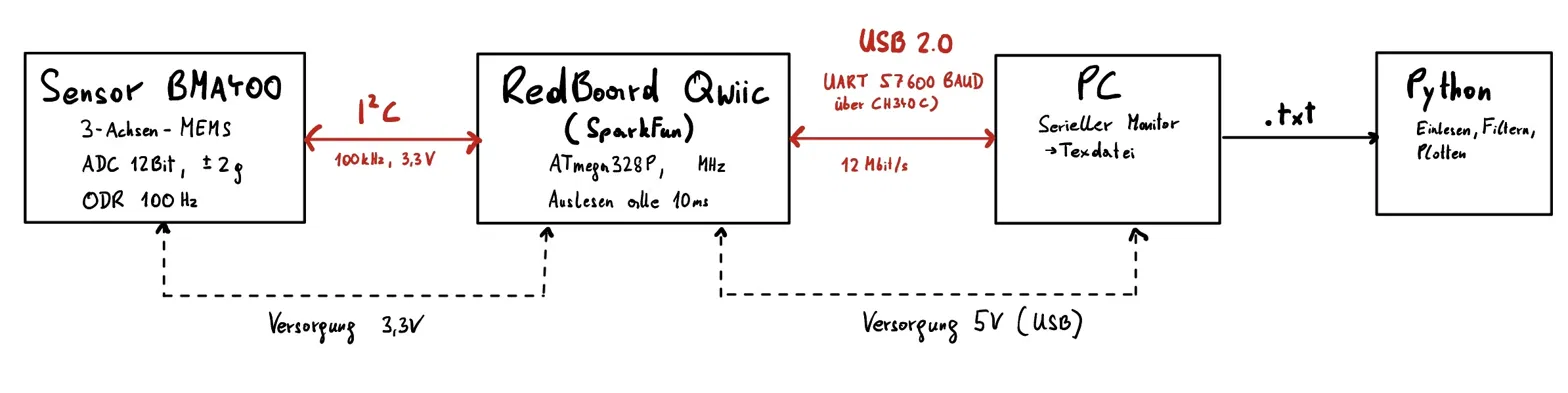
\includegraphics[width=\textwidth]{Messchaltung.png}
    \caption{Aufbau des stationären Messsystems (eigene Darstellung). Rot: Busse mit Typ und Geschwindigkeit, schwarz: Datenpfad zu Python, gestrichelt: Spannungsversorgung.}
    \label{fig:messsystem}
\end{figure}

\textbf{Komponenten:}
\begin{description}
    \item[BMA400 (SparkFun Breakout \cite{sparkfun}):] Digitaler 3-Achsen-MEMS-Beschleunigungssensor mit
    12~Bit Auflösung. Messbereich ($\pm 2$ bis $\pm 16\,g$) und Datenrate (ODR, 12{,}5--800\,Hz)
    sind einstellbar; die Messwerte stehen in den Registern 0x04--0x09 \cite{bma400}.
    \item[SparkFun RedBoard Qwiic (ATmega328P, 16\,MHz, Arduino-Uno-kompatibel):] Konfiguriert den Sensor, liest die sechs
    Datenregister aus, rechnet die Rohwerte in $g$ um und hängt den Zeitstempel
    \texttt{millis()} an. Er versorgt den Sensor mit 3{,}3\,V.
    \item[PC (Arduino IDE):] Der serielle Monitor zeigt die Messwerte zeilenweise
    (\texttt{X Y Z Time}) an; sie werden per Copy \& Paste in eine \texttt{.txt}-Datei
    übernommen.
    \item[Python (\texttt{MainCode1.ipynb}):] Liest die Textdatei mit \texttt{pandas} ein,
    filtert mit \texttt{SciPy} \cite{scipy} und stellt die Daten mit \texttt{matplotlib} dar.
\end{description}

\textbf{Busse und Signalpfade:}
\begin{description}
    \item[I\textsuperscript{2}C (100\,kHz):] Zweidraht-Bus (SDA = A4, SCL = A5). Der Arduino ist
    Master, der Sensor Slave mit der Adresse 0x14.
    \item[UART / USB 2.0:] Der Arduino sendet seriell mit 57\,600\,Baud; der USB-Seriell-Wandler
    CH340C auf dem Board setzt dies auf USB 2.0 Full Speed (12\,Mbit/s) um.
    \item[Datenpfad PC $\rightarrow$ Python:] Übergabe der Messdaten als Textdatei.
    \item[Spannungsversorgung:] 5\,V über USB für den Arduino, 3{,}3\,V und GND vom Arduino
    zum Sensor.
\end{description}

\subsection{Mobiles Messsystem}

Für Aufgabe~9 wird der USB-Anschluss durch einen DataLogger und eine Batterie
ersetzt. Laut \texttt{Lab1Code2} besteht das mobile System aus dem Arduino, dem
Beschleunigungssensor \textbf{MMA8452Q} (SparkFun, $\pm 8\,g$, ODR 200\,Hz) und
einem \textbf{Qwiic OpenLog} (SparkFun) mit microSD-Karte. Sensor und OpenLog hängen
beide am I\textsuperscript{2}C-Bus des Arduino (OpenLog-Adresse 42); der Arduino
sendet jede Messzeile per I\textsuperscript{2}C an den OpenLog, der sie in die Datei
\texttt{ACCdata.txt} auf der SD-Karte schreibt. Die Datei wird danach am PC
ausgewertet. Die Spannungsversorgung übernimmt statt USB eine 9-V-Alkali-Batterie
(Blockbatterie 6LR61); der Spannungsregler des Arduino erzeugt daraus 5\,V bzw.\ 3{,}3\,V.

% =====================================================================
\section{Vorausgehende Arbeiten}
% =====================================================================

\subsection{Messstrategie}

\begin{itemize}
  \item \textbf{Dynamische Messung:} schnelle Auf- und Abbewegung (ca.\ 1\,Hz) zuerst mit
        dem Originalcode (ODR 12{,}5\,Hz), dann mit erhöhter ODR (Aufgaben 4 und 5).
  \item \textbf{Statische Messung:} Sensor nacheinander in allen sechs Lagen je ca.\ 10\,s
        ruhig halten, um Achsenzuordnung, Vorzeichen und Betrag ($\approx 1\,g$) zu prüfen
        (Aufgabe 6).
  \item \textbf{Zeitbasis:} Zeitstempel \texttt{millis()} direkt auf dem Arduino, daraus
        Bestimmung der tatsächlichen Abtastfrequenz (Aufgaben 8 und 9).
\end{itemize}

\subsection{Umrechnung eines ADC-Wertes in eine Temperatur (Aufgabe 2)}

Gegeben sind ein Temperatursensor mit $U = 0 \ldots 3{,}3$\,V für
$\vartheta = 0 \ldots 40\,^\circ$C (linear) und ein ADC mit $n = 10$\,Bit
($0 \ldots 1023$) und Referenzspannung $U_\mathrm{ref} = 5$\,V. Der ADC liefert
$D = 520$.

\textbf{Schritt 1 -- ADC-Wert in Spannung:}
\begin{equation}
  U = \frac{D}{2^{n}-1}\cdot U_\mathrm{ref} = \frac{520}{1023}\cdot 5\,\mathrm{V} \approx 2{,}542\,\mathrm{V}
\end{equation}

\textbf{Schritt 2 -- Spannung in Temperatur:}
\begin{equation}
  \vartheta = \frac{U}{3{,}3\,\mathrm{V}}\cdot 40\,^\circ\mathrm{C}
            = \frac{2{,}542\,\mathrm{V}}{3{,}3\,\mathrm{V}}\cdot 40\,^\circ\mathrm{C}
            \approx \mathbf{30{,}8\,^\circ C}
\end{equation}

Der Sensor misst also ca.\ 30{,}8\,°C, was für eine Messung auf der Haut plausibel
ist (die Hauttemperatur liegt unter der Körperkerntemperatur von ca.\ 37\,°C).
Da der Sensor höchstens 3{,}3\,V liefert, werden nur ADC-Werte bis
$\frac{3{,}3}{5}\cdot 1023 \approx 675$ genutzt; die Auflösung beträgt damit
$40\,^\circ\mathrm{C}/675 \approx 0{,}06\,^\circ$C pro Stufe statt der möglichen
$0{,}04\,^\circ$C.

\subsection{Achsenzuordnung und Umrechnung in physikalische Größen (Aufgabe 3)}

\textbf{Achsenzuordnung:} \texttt{Lab1Code1} gibt pro Zeile \texttt{X Y Z Time}
aus; die Spalten entsprechen der Reihenfolge der Datenregister (0x04/0x05 = $x$,
0x06/0x07 = $y$, 0x08/0x09 = $z$) und damit den auf der Platine aufgedruckten Achsen.

\textbf{Test:} Der Sensor wird so hingelegt, dass eine Achse senkrecht nach oben
zeigt. Diese Achse zeigt dann ca.\ $+1\,g$, die anderen ca.\ $0\,g$. Flach auf dem
Tisch ($z$ nach oben) wurde z.\,B.\ \texttt{7 -91 1002} gemessen, also $z \approx 1\,g$.
Die systematische Prüfung aller sechs Lagen erfolgt in Aufgabe~6.

\textbf{Einheit:} Ausgegeben werden Rohwerte in LSB (Digits): pro Achse zwei
Register (LSB, MSB), die zusammen einen 12-Bit-Wert im Zweierkomplement
($-2048 \ldots +2047$) ergeben:
\texttt{raw = ((msb \& 0x0F) << 8) | lsb}, danach bei \texttt{raw > 2047}
$\rightarrow$ \texttt{raw -= 4096}.

\textbf{Umrechnung:} Die Empfindlichkeit ergibt sich laut Datenblatt \cite{bma400} (S.~10, Tabelle \emph{Output Signal}) zu
$S = 2048/\text{Messbereich}$, also $S = 1024$\,LSB/$g$ bei $\pm 2\,g$:
\begin{equation}
  a\,[g] = \frac{\text{raw}}{1024}, \qquad
  a\,[\mathrm{m/s^2}] = \frac{\text{raw}}{1024}\cdot 9{,}81\,\mathrm{m/s^2}
\end{equation}
Beispiel: $1002/1024 = 0{,}98\,g = 9{,}60$\,m/s$^2$.

\subsection{Skripte}

Der Python-Code \texttt{MainCode1.ipynb} bearbeitet die Aufgaben 4\,(a), 5,
6\,(a), 7, 8 und 9 und erzeugt alle Abbildungen dieses Berichts. Der Arduino-Code
wurde für Aufgabe~5 angepasst (\texttt{Lab1Code1\_modifiziert.ino}). Beide Dateien
liegen der Abgabe bei (Anhang~\ref{sec:anhang}).

% =====================================================================
\section{Beantwortung der Aufgabenstellung}
% =====================================================================

\subsection{Auf- und Abbewegung mit dem Originalcode (Aufgabe 4)}

Der Sensor wurde ohne Rotation bewegt und die Daten mit \texttt{Lab1Code1}
(ODR 12{,}5\,Hz, $\pm 2\,g$) aufgezeichnet und in eine Textdatei kopiert.

\textbf{(a)} Abbildung~\ref{fig:a4} zeigt 4\,s der Messung, umgerechnet in $g$.

\begin{figure}[H]
  \centering
  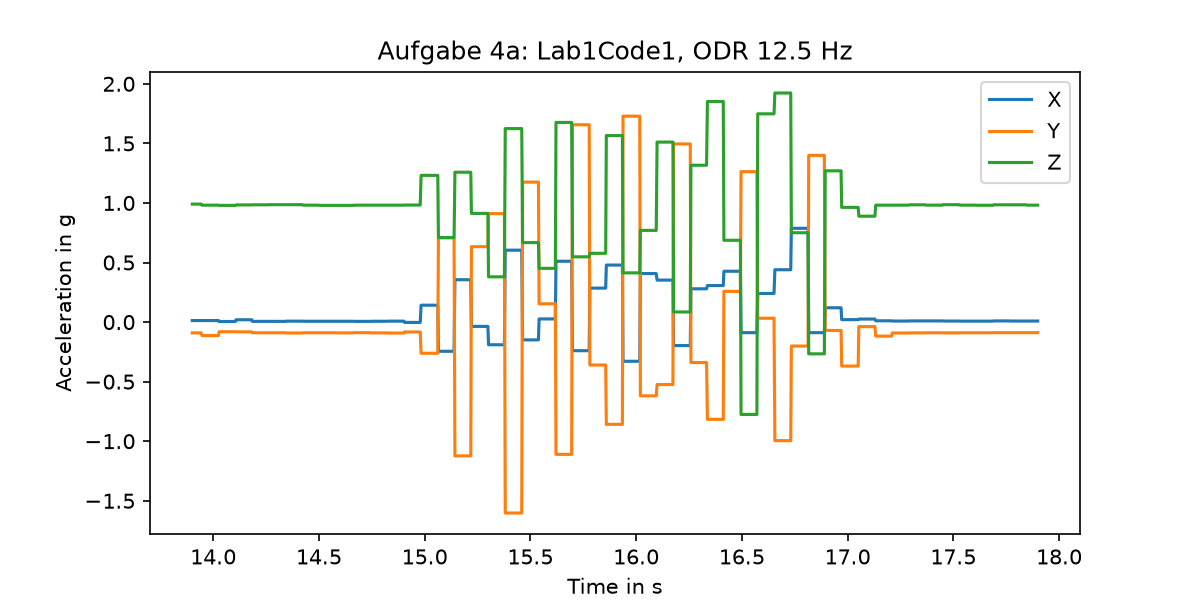
\includegraphics[width=0.85\textwidth]{A4a_12_5Hz.png}
  \caption{Auf- und Abbewegung mit \texttt{Lab1Code1} (ODR 12{,}5\,Hz), Ausschnitt 4\,s.}
  \label{fig:a4}
\end{figure}

\textbf{(b) Plateaus der Peaks:} Jeder Wert bleibt ca.\ 80\,ms konstant, wodurch
die treppenförmigen Plateaus entstehen. Der Sensor liefert neue Werte nur mit der
ODR von 12{,}5\,Hz (alle 80\,ms), die \texttt{loop()} gibt ohne \texttt{delay}
jedoch ca.\ alle 3\,ms ($\approx 313$\,Hz, vgl.\ Tab.~\ref{tab:fs}) eine Zeile aus.
Bis ein neuer Wert im Datenregister steht, wird also immer wieder derselbe Wert
gelesen (ca.\ 25 identische Zeilen pro Messwert). \textbf{Lösung:} Die ODR im
Register \texttt{ACC\_CONFIG1} erhöhen (Aufgabe~5) und die Ausgaberate mit einem
passenden \texttt{delay} an die ODR anpassen. Zusätzlich liegen die Peaks in $z$
(inkl.\ Erdbeschleunigung) mit ca.\ $1{,}9\,g$ nahe an der Messbereichsgrenze von
$\pm 2\,g$; für stärkere Bewegungen sollte daher auch der Messbereich vergrößert
werden, um Sättigung zu vermeiden.

\textbf{(c) Abweichung von der tatsächlichen Bewegung:} Bei 12{,}5\,Hz liegt die
Nyquist-Frequenz bei 6{,}25\,Hz. Die schnelle Bewegung enthält höhere
Frequenzanteile, sodass \emph{Aliasing} entsteht: Pro Bewegung gibt es nur wenige
Messpunkte, das Signal springt (v.\,a.\ in $y$) fast bei jedem Sample das Vorzeichen,
statt den Bewegungsverlauf zu zeigen. Außerdem misst der Sensor immer die
Erdbeschleunigung mit; dreht sich die Hand leicht, verteilt sich diese auf
mehrere Achsen.

\subsection{Anpassung der Sensorkonfiguration (Aufgabe 5)}

Die neue Messung wurde mit dem Beschleunigungssensor MMA8452Q durchgeführt, für den
\texttt{Lab1Code1} ursprünglich geschrieben ist (Messbereich $\pm 2\,g$, Datenrate
1{,}56\,Hz). Laut Datenblatt MMA8452Q \cite{mma8452q} wird die Datenrate im Register
\texttt{CTRL\_REG1} (0x2A) über den Parameter \texttt{DR[2:0]} (Bits 5:3)
eingestellt (S.~37, Tab.~53 und 55). Die möglichen Werte zeigt Tab.~\ref{tab:odr}.
Zusätzlich wurde der Messbereich im Register \texttt{XYZ\_DATA\_CFG} (0x0E) über
\texttt{FS[1:0]} (Bits 1:0) geändert (S.~22, Tab.~15 und 16): 00 = $\pm 2\,g$, 01 = $\pm 4\,g$,
10 = $\pm 8\,g$, 11 = reserviert.

\begin{table}[H]
\centering
\small
\caption{Mögliche Werte des Parameters \texttt{DR[2:0]} im Register \texttt{CTRL\_REG1} (0x2A) des MMA8452Q.}
\label{tab:odr}
\begin{tabular}{lcccccccc}
\toprule
\texttt{DR[2:0]} & 000 & 001 & 010 & \textbf{011} & 100 & 101 & 110 & 111 \\
\midrule
ODR / Hz & 800 & 400 & 200 & \textbf{100} & 50 & 12{,}5 & 6{,}25 & 1{,}56 \\
\bottomrule
\end{tabular}
\end{table}

Im Code (\texttt{Lab1Code1\_modifiziert.ino}) wurden folgende Zeilen geändert:
\begin{lstlisting}
accel.setScale(SCALE_8G);     // XYZ_DATA_CFG (0x0E), FS = 10, vorher SCALE_2G
accel.setDataRate(ODR_100);   // CTRL_REG1 (0x2A), DR = 011, vorher ODR_1 (1,56 Hz)
\end{lstlisting}
In \texttt{loop()} wird nur ausgegeben, wenn der Sensor einen neuen Wert hat
(\texttt{accel.available()}). Die Rohwerte werden in Python mit 256\,LSB/$g$
(12\,Bit bei $\pm 8\,g$) in $g$ umgerechnet.

\textbf{Begründung:} Handbewegungen liegen deutlich unter 50\,Hz (Nyquist-Frequenz
bei 100\,Hz) und werden damit ohne Aliasing erfasst. Höhere Raten sind nicht nötig
und belasten nur die Übertragung: Eine Ausgabezeile (z.\,B.\
\texttt{-23\textbackslash t3\textbackslash t-252\textbackslash t41000}
+ Zeilenumbruch) umfasst ca.\ 20 Zeichen $\approx 200$\,Bit, bei 57\,600\,Baud sind
also nur ca.\ 290 Zeilen/s übertragbar -- ab 400\,Hz wäre die serielle Schnittstelle
überlastet. Der Messbereich $\pm 8\,g$ verhindert, dass schnelle Bewegungen über
$2\,g$ abgeschnitten werden (Sättigung); dafür sinkt die Auflösung auf
$1/256\,g \approx 4\,mg$, was für Handbewegungen ausreicht.

\begin{figure}[H]
  \centering
  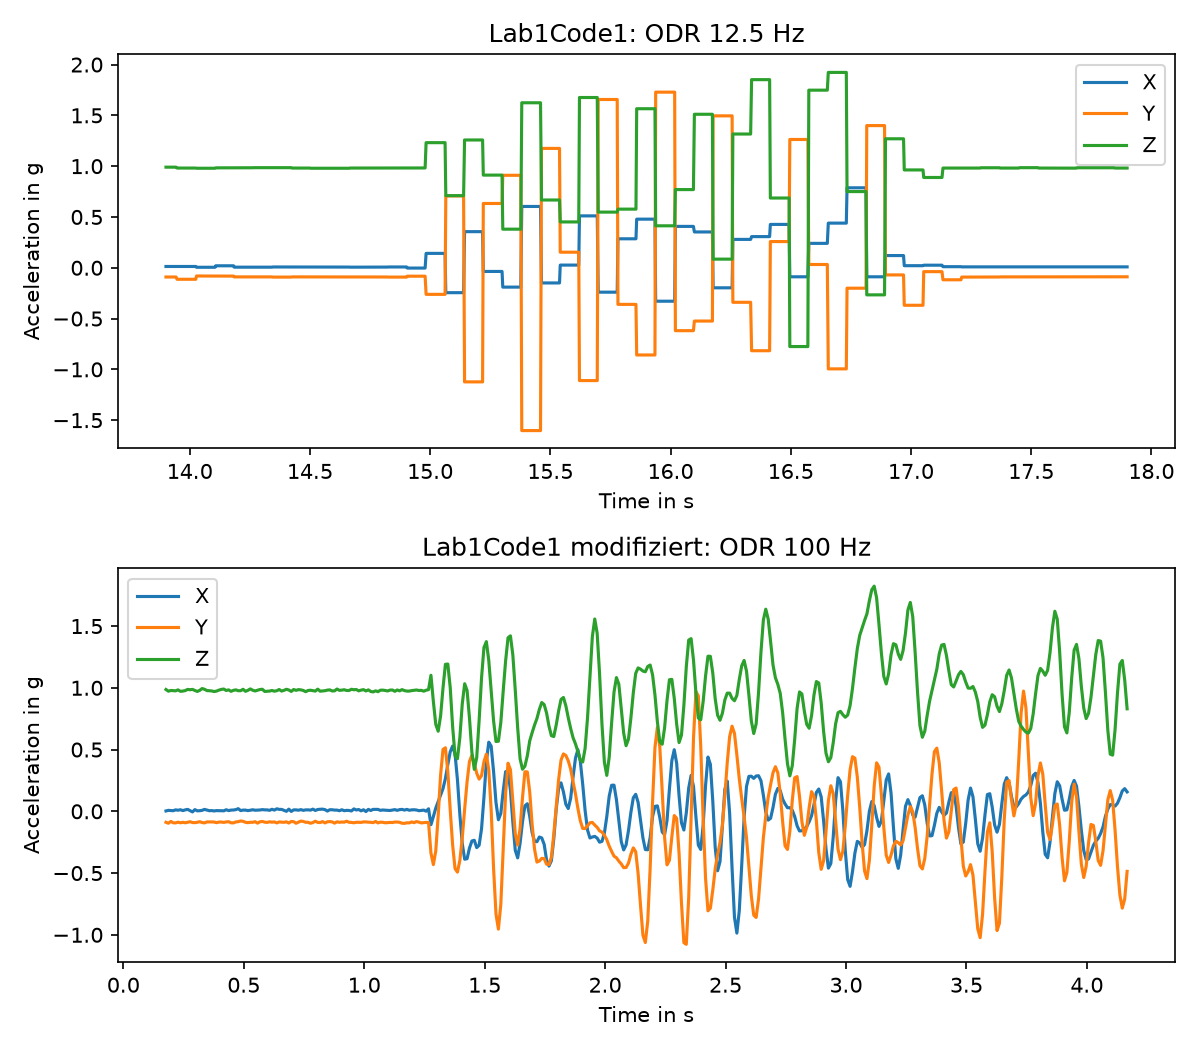
\includegraphics[width=0.72\textwidth]{A5_Vergleich_12_5Hz_100Hz.png}
  \caption{Vergleich je 4\,s: oben A4 mit ODR 12{,}5\,Hz (BMA400), unten A5 mit ODR 100\,Hz und $\pm 8\,g$ (MMA8452Q, modifizierter Code).}
  \label{fig:a5}
\end{figure}

\textbf{Vergleich (Abb.~\ref{fig:a5}):} Die Messung aus Aufgabe~4 wurde mit dem
BMA400 (ODR 12{,}5\,Hz), die neue Messung mit dem MMA8452Q (ODR 100\,Hz) aufgenommen;
da beide in $g$ umgerechnet sind, sind die Werte direkt vergleichbar. Gemeinsam ist
beiden der Ruhepegel mit einem Betrag von ca.\ $1\,g$ in $z$-Richtung ($x$ und
$y \approx 0$); in der neuen Messung lag der Sensor umgedreht, daher
$z \approx -1\,g$. Bei 100\,Hz gibt es keine Treppenstufen mehr: Die Kurve ist glatt
und die einzelnen Auf-ab-Bewegungen (ca.\ 1--2 pro Sekunde) sind als Schwingung um
den Ruhepegel zu erkennen, während das Signal bei 12{,}5\,Hz durch das Aliasing
zerhackt ist. Die Ausschläge sind in der neuen Messung kleiner (meist
$\pm 0{,}5\,g$), weil die Bewegung weniger heftig war. Einzelne Spitzen bis ca.\
$-3\,g$, die nur ein Sample lang sind, sind vermutlich Stöße bzw.\ Ausreißer; sie
werden dank $\pm 8\,g$ nicht abgeschnitten. Wesentlicher Unterschied ist also die
höhere Abtastrate.

\subsection{Zeitstempel und statische Messung in sechs Orientierungen (Aufgabe 6)}

Jede Zeile erhält direkt auf dem Arduino den Zeitstempel \texttt{millis()}
(4.~Spalte), unabhängig von den Zeitstempeln des seriellen Monitors. Daraus wird in
Abschnitt~\ref{sec:fs} die mittlere Abtastfrequenz berechnet.

\textbf{(a)} Abbildung~\ref{fig:a6} zeigt die gesamte Messung.

\begin{figure}[H]
  \centering
  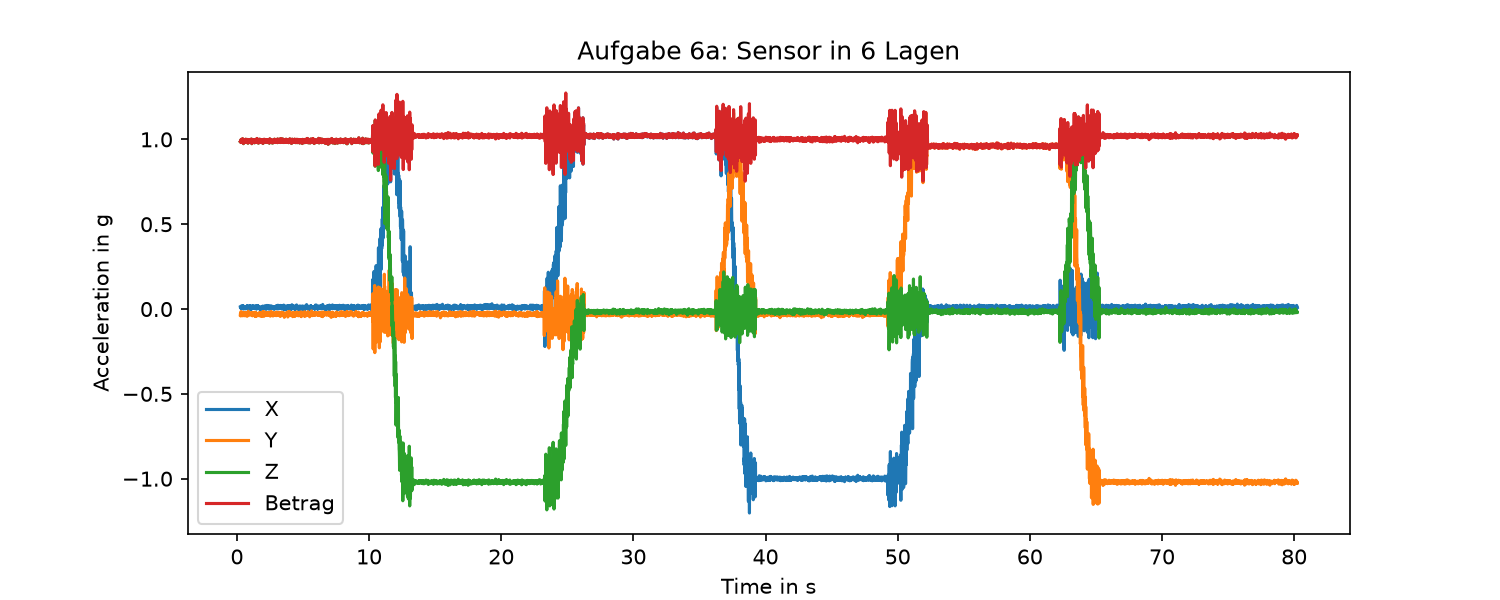
\includegraphics[width=0.9\textwidth]{A6a_6_Lagen.png}
  \caption{Sensor in sechs Lagen à ca.\ 10\,s; rot: Betrag $|a| = \sqrt{x^2+y^2+z^2}$.}
  \label{fig:a6}
\end{figure}

\textbf{(b) Plausibilität:} Tabelle~\ref{tab:lagen} zeigt die Mittelwerte in den
Ruhephasen.

\begin{table}[H]
\centering
\small
\caption{Mittelwerte der Beschleunigung in den sechs Lagen (Werte in $g$).}
\label{tab:lagen}
\begin{tabular}{lcccc}
\toprule
Lage & $x$ & $y$ & $z$ & $|a|$ \\
\midrule
$z$ oben  & 0{,}01 & $-0{,}03$ & \textbf{0{,}99} & 0{,}99 \\
$z$ unten & 0{,}01 & $-0{,}03$ & \textbf{$-$1{,}02} & 1{,}02 \\
$x$ oben  & \textbf{1{,}02} & $-0{,}03$ & $-0{,}02$ & 1{,}02 \\
$x$ unten & \textbf{$-$1{,}00} & $-0{,}03$ & $-0{,}02$ & 1{,}00 \\
$y$ oben  & 0{,}01 & \textbf{0{,}96} & $-0{,}02$ & 0{,}96 \\
$y$ unten & 0{,}01 & \textbf{$-$1{,}02} & $-0{,}02$ & 1{,}02 \\
\bottomrule
\end{tabular}
\end{table}

Die Daten ergeben Sinn: Die senkrecht stehende Achse zeigt immer ca.\ $\pm 1\,g$,
die anderen ca.\ $0\,g$, und der Betrag liegt stets bei ca.\ $1\,g$. Zeigt eine Achse
nach oben, ist der Wert positiv, weil der Sensor die Gegenkraft der Unterlage
misst. Die kleinen Abweichungen (bis 0{,}04\,$g$) entstehen durch Offset-Fehler
des Sensors und dadurch, dass er von Hand nicht exakt gerade gehalten wurde.

\subsection{Filterung der Daten (Aufgabe 7)}

Die Daten aus Aufgabe~6 wurden mit einem Butterworth-Tiefpass 4.~Ordnung mit der
Grenzfrequenz $f_g = 5$\,Hz gefiltert. Dabei wurde \texttt{filtfilt()} aus
\texttt{scipy.signal} \cite{scipy} verwendet, das den Filter vorwärts und rückwärts
anwendet und so keine Phasenverschiebung erzeugt (Nullphasenfilter).

\begin{figure}[H]
  \centering
  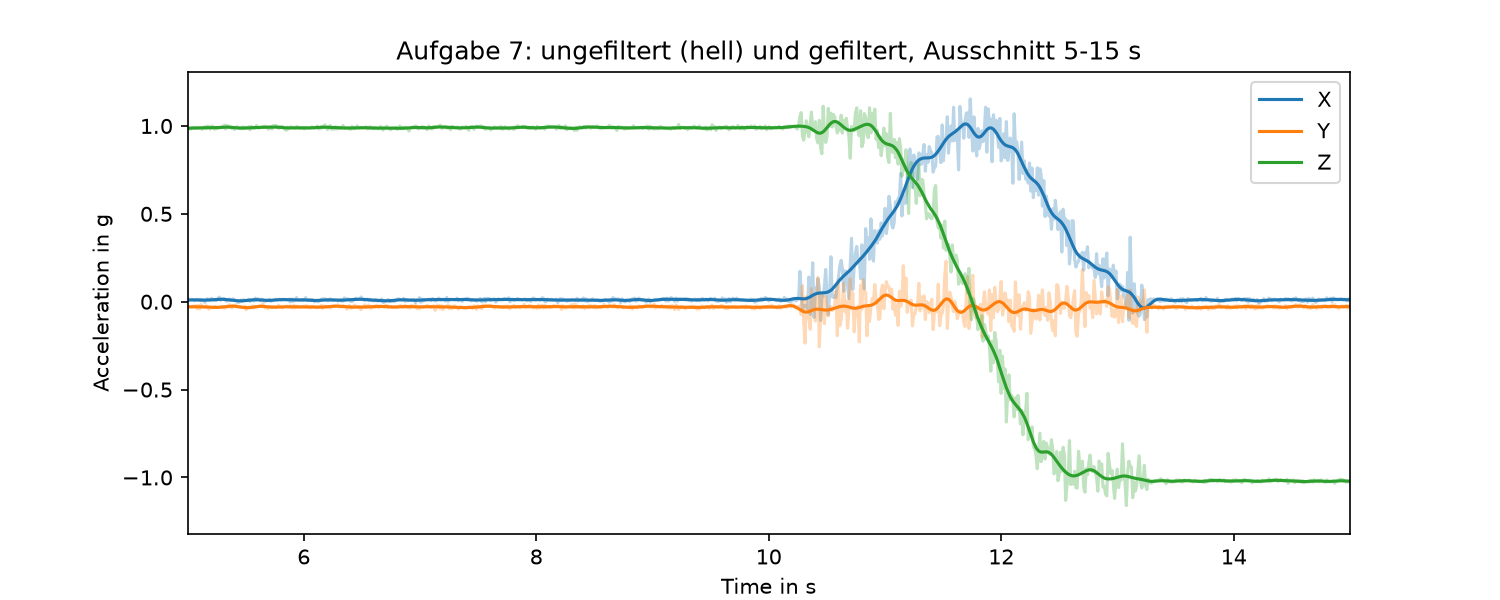
\includegraphics[width=0.9\textwidth]{A7_Filter.png}
  \caption{Ungefilterte (hell) und tiefpassgefilterte Daten ($f_g = 5$\,Hz), Ausschnitt 5--15\,s.}
  \label{fig:a7}
\end{figure}

\textbf{Effekt und Begründung:} Der Filter entfernt das Sensorrauschen und das
Zittern der Hand (in Ruhe sinkt die Standardabweichung von $z$ von 6{,}0 auf
1{,}6\,m$g$), während die Lagewechsel erhalten bleiben und durch \texttt{filtfilt}
nicht verschoben werden (Abb.~\ref{fig:a7}). Ein Tiefpass wurde gewählt, weil sich
die Lage nur langsam ändert, das Rauschen aber hochfrequent ist.

\subsection{Bestimmung der Abtastfrequenz (Aufgabe 8)}
\label{sec:fs}

Aus den \texttt{millis()}-Zeitstempeln wurden die Abtastintervalle
$\Delta t_i = t_{i+1}-t_i$ und daraus
\begin{equation}
  \bar f_s = \frac{1}{\overline{\Delta t}}, \qquad
  \sigma_{f_s} \approx \frac{\sigma_{\Delta t}}{\overline{\Delta t}^{\,2}}
\end{equation}
bestimmt (Fehlerfortpflanzung). Abbildung~\ref{fig:a8} zeigt die Verteilung der
Intervalle, Tab.~\ref{tab:fs} die Ergebnisse.

\begin{figure}[H]
  \centering
  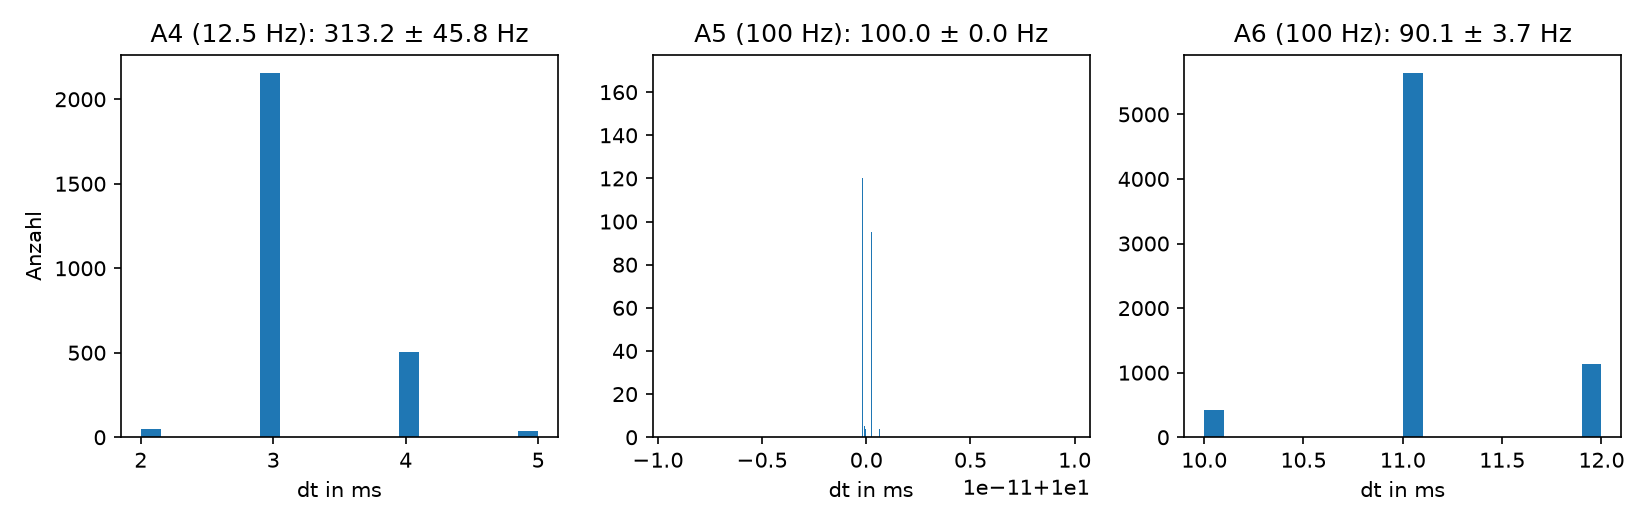
\includegraphics[width=\textwidth]{A8_Abtastfrequenz.png}
  \caption{Histogramme der Abtastintervalle $\Delta t$ der drei Messungen.}
  \label{fig:a8}
\end{figure}

\begin{table}[H]
\centering
\small
\caption{Abtastintervalle und Abtastfrequenzen der Messungen.}
\label{tab:fs}
\begin{tabular}{lccc}
\toprule
Messung & $\overline{\Delta t}$ / ms & $\sigma_{\Delta t}$ / ms & $\bar f_s$ / Hz \\
\midrule
A4: \texttt{Lab1Code1} (ODR 12{,}5\,Hz)        & 3{,}19  & 0{,}47 & $313 \pm 46$ \\
A5: modifiziert (ODR 100\,Hz)                   & 9{,}91  & 0{,}65 & $100{,}9 \pm 6{,}6$ \\
A6: 6 Lagen (ODR 100\,Hz)                       & 11{,}10 & 0{,}46 & $90{,}1 \pm 3{,}7$ \\
A9: mobiles System (\texttt{Lab1Code2})         & 18{,}79 & 0{,}95 & $53{,}2 \pm 2{,}7$ \\
\bottomrule
\end{tabular}
\end{table}

Bei \texttt{Lab1Code1} (A4) gibt die Schleife ohne \texttt{delay} mit ca.\ 313\,Hz
aus, neue Sensorwerte kommen aber nur mit 12{,}5\,Hz. Im modifizierten Code (A5)
wird nur bei einem neuen Sensorwert ausgegeben (\texttt{available()}), der Takt
kommt also vom Sensor: Die Abtastfrequenz liegt mit $100{,}9 \pm 6{,}6$\,Hz bei der
eingestellten ODR. Dass sie leicht über 100\,Hz liegt, liegt an der Toleranz des
internen Oszillators des Sensors; die Streuung (9--11\,ms) entsteht vor allem durch
die Auflösung von \texttt{millis()} von 1\,ms. In Messung A6 (BMA400, Takt über
\texttt{delay(10)}) liegt sie dagegen bei 90\,Hz, weil zu \texttt{delay(10)} noch die
Zeit für das Auslesen über I\textsuperscript{2}C und \texttt{Serial.print}
hinzukommt ($\Delta t \approx 11$\,ms). Die Taktung über den Sensor ist daher
genauer. Für eine feinere Bestimmung wäre \texttt{micros()} besser geeignet.

\subsection{Mobiles Messsystem (Aufgabe 9)}

Mit dem mobilen Messsystem (MMA8452Q, Qwiic OpenLog mit SD-Karte, Batterie) wurden mit
\texttt{Lab1Code2} 545 Werte über 10{,}2\,s aufgezeichnet
(\texttt{IMU\_A9\_mobil\_Lab1Code2.txt}). Der Sensor lag dabei überwiegend ruhig und
leicht geneigt, nur bei ca.\ 2--3\,s wurde er kurz bewegt. Der Betrag der
Beschleunigung liegt im Mittel bei $0{,}986\,g$, die Daten sind also plausibel
(Abb.~\ref{fig:a9}, links). Die Abtastfrequenz wurde wie in Abschnitt~\ref{sec:fs}
bestimmt und mit der stationären Messung A6 (BMA400, ODR 100\,Hz, USB)
verglichen (Abb.~\ref{fig:a9}, rechts, und Tab.~\ref{tab:fs}). \texttt{Lab1Code2} rechnet die Rohwerte bereits in $g$ um (256\,LSB/$g$ bei $\pm 8\,g$).

\begin{figure}[H]
  \centering
  \includegraphics[width=\textwidth]{A9_mobil.png}
  \caption{Mobiles Messsystem mit \texttt{Lab1Code2}: links die Messdaten (10\,s),
  rechts die Verteilung der Abtastintervalle im Vergleich zur stationären Messung A6.}
  \label{fig:a9}
\end{figure}

\textbf{Ergebnis:} Das mobile System tastet mit
$\bar f_s = 53{,}2 \pm 2{,}7$\,Hz ab ($\overline{\Delta t} = 18{,}79 \pm 0{,}95$\,ms,
Bereich 17--24\,ms), das stationäre mit $90{,}1 \pm 3{,}7$\,Hz
($\overline{\Delta t} = 11{,}10 \pm 0{,}46$\,ms, Bereich 10--12\,ms). Die
Abtastfrequenz ist mobil also um ca.\ 40\,\% kleiner, und die Intervalle streuen
absolut etwa doppelt so stark, mit einzelnen Ausreißern bis 24\,ms.

\textbf{Diskussion:} Die Abtastfrequenz wird nicht von der ODR des Sensors bestimmt,
sondern von der Dauer eines Schleifendurchlaufs auf dem Mikrocontroller. Der
MMA8452Q läuft in \texttt{Lab1Code2} mit 200\,Hz, es wird also nur etwa jeder vierte
mögliche Wert erfasst. In jedem Durchlauf liest der Arduino Status und $x$, $y$, $z$
einzeln über I\textsuperscript{2}C aus, ruft \texttt{myLog.append()} auf (öffnet die
Datei bei jedem Wert neu) und überträgt die ganze Textzeile in fünf
\texttt{print}-Aufrufen ebenfalls über I\textsuperscript{2}C an den OpenLog. Dieser
Bus (Standard 100\,kHz) ist deutlich langsamer als die serielle Ausgabe an den PC,
und der OpenLog braucht zusätzlich Zeit zum Verarbeiten und blockweisen Schreiben auf
die SD-Karte. Diese Zeit schwankt, daher streuen die Intervalle stärker und es gibt
einzelne Ausreißer bis 24\,ms. Außerdem unterscheidet sich der Aufbau insgesamt:
anderer Sensor (MMA8452Q statt BMA400), anderer Messbereich ($\pm 8\,g$,
256\,LSB/$g$) und Ausgabe mit nur zwei Nachkommastellen (Auflösung $0{,}01\,g$).
Zeitstempel und Takt kommen aber in beiden Fällen vom Arduino (\texttt{millis()},
1\,ms Auflösung), sodass die Abtastfrequenzen direkt vergleichbar sind. Insgesamt
bestimmt die langsamste Stelle der Signalkette die tatsächliche Abtastfrequenz;
die ODR ist nur eine Obergrenze.

% =====================================================================
\section{Zusammenfassung}
% =====================================================================
Das Messsystem aus Beschleunigungssensor (BMA400 bzw.\ MMA8452Q), Arduino und PC
wurde aufgebaut und in Betrieb genommen. Mit der Standardkonfiguration (ODR
12{,}5\,Hz) bildeten die Daten die schnelle Bewegung wegen zu geringer Abtastrate
(Aliasing) und mehrfach ausgegebener Werte nicht korrekt ab. Durch Erhöhen der ODR
auf 100\,Hz (\texttt{CTRL\_REG1} des MMA8452Q) und des Messbereichs auf $\pm 8\,g$
wurde die Bewegung korrekt erfasst (Abtastfrequenz $100{,}9 \pm 6{,}6$\,Hz). Die statische Messung
bestätigte in allen sechs Lagen eine Beschleunigung von ca.\ $1\,g$ (Abweichung
$\leq 0{,}04\,g$). Ein Butterworth-Tiefpass (5\,Hz, \texttt{filtfilt}) reduzierte das
Rauschen deutlich ohne Phasenverschiebung. Die tatsächliche Abtastfrequenz betrug
ca.\ 90\,Hz (stationär) bzw.\ 53\,Hz (mobil, \texttt{Lab1Code2} mit DataLogger).

\bibliographystyle{IEEEtran}
\bibliography{Literatur}

\textbf{Hinweis zur Verwendung von KI:} Bei der Erstellung dieses Berichts und des
Python-Codes wurden KI-Werkzeuge (Claude, Anthropic) als Hilfsmittel für die
Formulierung von Texten sowie für Code und Fehlersuche eingesetzt. Alle Messungen
wurden selbst durchgeführt; Ergebnisse und Inhalte wurden von der Gruppe geprüft.

% =====================================================================
\appendix
\section{Anhang: Abgegebene Dateien (Aufgabe 10)}
\label{sec:anhang}
% =====================================================================
Die Abgabe \texttt{Lab1\_Gruppe\_4.zip} enthält:
\begin{itemize}
  \item \texttt{Bericht\_1\_Gruppe\_4.pdf} -- dieser Bericht,
  \item \texttt{Lab1Code1\_modifiziert.ino} -- modifizierter Arduino-Code (Aufgabe 5),
  \item \texttt{MainCode1.ipynb} -- Python-Auswertung (Aufgaben 4a, 5, 6a, 7, 8, 9); läuft komplett durch und speichert alle Abbildungen in \texttt{figures/},
  \item Datensätze in \texttt{data/}: \texttt{IMU\_A4\_Lab1Code1\_roh.csv}, \texttt{IMU\_A5\_Lab1Code1mod\_100Hz.csv}, \texttt{IMU\_A6\_Lagen.csv}, \texttt{IMU\_A9\_mobil\_Lab1Code2.txt}.
\end{itemize}

\end{document}
